% This is samplepaper.tex, a sample chapter demonstrating the
% LLNCS macro package for Springer Computer Science proceedings;
% Version 2.20 of 2017/10/04
%
\documentclass[runningheads]{llncs}
%
\usepackage{amsmath}
\usepackage{booktabs} % For pretty tables
\usepackage{caption} % For caption spacing
\usepackage{graphicx}
\usepackage{pgfplots}
\usepackage[all]{nowidow}
\usepackage[utf8]{inputenc}
\usepackage{tikz}
\usetikzlibrary{er,positioning,bayesnet}
\usepackage{multicol}
\usepackage{algpseudocode,algorithm,algorithmicx}
\usepackage{hyperref}
\usepackage[inline]{enumitem} % Horizontal lists
% Used for displaying a sample figure. If possible, figure files should
% be included in EPS format.
%
% If you use the hyperref package, please uncomment the following line
% to display URLs in blue roman font according to Springer's eBook style:
% \renewcommand\UrlFont{\color{blue}\rmfamily}

\newcommand{\card}[1]{\left\vert{#1}\right\vert}
\newcommand*\Let[2]{\State #1 $\gets$ #2}

\pgfplotsset{compat=1.14}

\renewcommand{\topfraction}{0.85}
\renewcommand{\bottomfraction}{0.85}
\renewcommand{\textfraction}{0.15}
\renewcommand{\floatpagefraction}{0.8}
\renewcommand{\textfraction}{0.1}
\setlength{\floatsep}{3pt plus 1pt minus 1pt}
\setlength{\textfloatsep}{3pt plus 1pt minus 1pt}
\setlength{\intextsep}{3pt plus 1pt minus 1pt}
\setlength{\abovecaptionskip}{2pt plus 1pt minus 1pt}


\begin{document}
%
\title{A thermodynamically consistent multi-phase model of Extracellular Matrix}
%
\titlerunning{Mechanical Properties of ECM}
% If the paper title is too long for the running head, you can set
% an abbreviated paper title here
%
\author{Giulia Laura Celora}
%
%\authorrunning{F. Author et al.}
% First names are abbreviated in the running head.
% If there are more than two authors, 'et al.' is used.
%
\institute{Mathematical Institute University of Oxford}
%
\maketitle              % typeset the header of the contribution
%
\begin{abstract}

\end{abstract}
%
%
%
\section{Introduction}
There are now several studies supporting the central role of mechanical stimulus in tissue morphogenesis and homeostasis, alongside with biochemical signalling. \textit{In vitro} studies have shown that ECM rigidity and shear stresses can alone promote the transition to malignant phenotype of normal cells and consequently the growth of a tumour mass. Despite the well-known link between cell behaviour and mechanical stimuli, the lack of quantitative measurement has delayed our understanding of such phenomena. The development of new nanotechnology has now open to the possibility of measuring mechanical stresses by the use of external devices. Meanwhile, new techniques such as Atomic Force Microscopy (AFM) have been developed to measure the local mechanical properties of tissue, with atomic precision. Combining such information can boost our understanding and the development of a solid mathematical framework to describe tumour growth and exploit mechanics to improve and revolutionise current therapy against cancer. 

The aim of coupling micro-environment and cell behaviours requires a clear understanding of both and the investigation of phenomena occurring at different time and spacial scales. In this work we focus on the Extracellular Matrix (ECM), the external network of polymers supporting cells in tissues. Its mechanical properties, in particular its stiffness, contribute to determine the response of tissues to external mechanical stimuli. By controlling the composition of the matrix, its properties can be tuned to meet the function of a specific tissues. 

Experiments have shown that tumour development is associated to a stiffening of the tissue compared to the surrounding healthy one, despite the fact that tumour cells themselves are usually softer than normal ones. Such contradiction is just apparent, as ECM can account for such resistance to mechanical stimuli. As a result, cells are exposed to higher compressive stresses which can select for more aggressive and invasive phenotype of cancer cells, as well as favour the collapse of blood vessels and impede the diffusion of substances in the extra-cellular environment ultimately decreasing the efficacy of numerous therapies.

Usually approach to the modelling of solid tumour is the use of multi-phase theory, according to which tumour are equivalent to material consisting of a solid matrix of cells and ECM, and an interstitial fluid phase. Besides involving the use of fundamental laws such as conservation of mass and momentum, the formulation of the model requires the use of several constitutive equation for each of the phase considered. These dictate the macroscopic behaviour of the system and thus heavily affect the prediction of the model, and are usually based on experimental result and have thus a limited range of applicability. Having a more fundamental description of the system requires instead deriving such properties based on the microscopic behaviour of the system.   As mentioned before, there is little understanding on the properties of the fundamental components of the ECM.

\section{Extracellular Matrix.}
Despite the tissue-specific nature of Extracellular Matrix (ECM), this is mainly composed of a network of collagen fibrils entangled with charged chains of glycosaminoglycans (GAGs). While collagen is mainly responsible for the mechanical behaviour of the tissue, GAGs can imbibe water, giving ECM the ability to swell while maintaining its structural integrity. As a result, the ECM behave as a polyelectrolyte gel \cite{ecm,ecm2}. Besides being largely present in the natural world, synthetic polyelectrolytes are currently employed for a wide range of applications, such as drug delivery, biomedical devices, scaffolds for tissue engineering and soft robotics [ADD CITATIONS]. The increasing popularity of such material has boost the development of mathematical model of such systems, in particular focusing particularly on the their swelling and plastic behaviours [ADD CITATIONS].

There is now compelling evidence that the relaxation of stress in polymer gels, and thus in ECM is governed by the interplay of the poroelastic and viscoelastic nature of the gel. While the first determines the long range motion of solvents, visco-elastic dominates the stress relaxation dynamics at the microscopic level. Being the same level at which cells probe their environment, this suggests that the visco-elastic properties of the ECM might play a role in determining cell response [ADD ARTICLE IN NOTE AS CITATION].

\begin{figure}
	\centering
	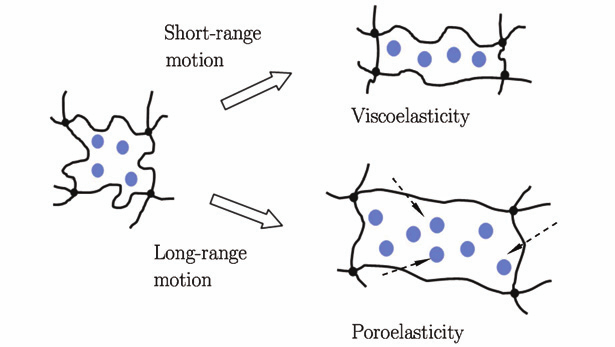
\includegraphics[scale=0.325]{latex/images/visco_poro}
	\caption{Illustration of the molecular processes which account for a gel deformation: viscosity is related to change in the conformation of the network which results in short-range movement of fluid relative to the polymers; poro-elasticity is instead responsible for the long-range diffusion of solvent molecules in the gel/tissue. Reproduced from \cite{viscoporo}.}
\end{figure}

The ECM is here considered as a three-phase medium composed of a solid polymer network with fixed charges, a solvent (i.e. water molecules) and solutes (freely moving charges).
\subsection{Balance Laws.}

Denote by $C_s$ the solvent concentration and by $C_i$ the concentration of mobile ions, $i=1,\ldots,N$. We assume that the only mechanism for the change in gel volume is the transport of solution, so that the molecular incompressibility condition must hold:



\bibliographystyle{splncs04}
\bibliography{biblio}
%
\end{document}
